% ****** Start of file apssamp.tex ******
%
%   This file is part of the APS files in the REVTeX 4.1 distribution.
%   Version 4.1r of REVTeX, August 2010
%
%   Copyright (c) 2009, 2010 The American Physical Society.
%
%   See the REVTeX 4 README file for restrictions and more information.
%
% TeX'ing this file requires that you have AMS-LaTeX 2.0 installed
% as well as the rest of the prerequisites for REVTeX 4.1
%
% See the REVTeX 4 README file
% It also requires running BibTeX. The commands are as follows:
%
%  1)  latex apssamp.tex
%  2)  bibtex apssamp
%  3)  latex apssamp.tex
%  4)  latex apssamp.tex
%
\documentclass[%
 reprint,
 twocolumn,
%superscriptaddress,
%groupedaddress,
%unsortedaddress,
%runinaddress,
%frontmatterverbose, 
%preprint,
%showpacs,preprintnumbers,
%nofootinbib,
%nobibnotes,
%bibnotes,
 amsmath,amssymb,
 aps,
%pra,
%prb,
%rmp,
%prstab,
%prstper,
floatfix,
]{revtex4}

\usepackage{graphicx}% Include figure files
\usepackage{dcolumn}% Align table columns on decimal point
\usepackage{bm}% bold math
%\usepackage{hyperref}% add hypertext capabilities
%\usepackage[mathlines]{lineno}% Enable numbering of text and display math
%\linenumbers\relax % Commence numbering lines

%\usepackage[showframe,%Uncomment any one of the following lines to test 
%scale=0.7, marginratio={1:1, 2:3}, ignoreall,% default settings
%text={7in,10in},centering,
%margin=1.5in,
%total={6.5in,8.75in}, top=1.2in, left=0.9in, includefoot,
%height=10in,a5paper,hmargin={3cm,0.8in},
%]{geometry}

\newcommand{\dd}{\mathrm{d}}


\newcommand{\Ecomment}[1]{\textcolor{red}{[E: #1]}}
\newcommand{\Dcomment}[1]{\textcolor{NavyBlue}{[D: #1]}}

%%%%%%%%%%%%%%%%%
\usepackage[usenames,dvipsnames]{xcolor}
%%%%%%%%%%%%%%%%%

\begin{document}

\preprint{APS/123-QED}

\title{A simple mechanism for higher-order correlations\\ in integrate-and-fire neurons}% Force line breaks with \\

\author{David A. Leen}
\email{dleen@washington.edu}

%Lines break automatically or can be forced with \\
 
\author{Eric Shea-Brown}%
\email{etsb@washington.edu}
\affiliation{%
Department of Applied Mathematics, University of Washington.
}

\date{\today}% It is always \today, today,
             %  but any date may be explicitly specified

\begin{abstract}
Here we show that a population of exponential integrate-and-fire (EIF) neurons receiving common input cannot be well described by a pairwise maximum entropy model. Common input into the EIF population hence gives rise to higher-order correlations. A tractable reduction of the EIF model, the linear-nonlinear (LN) cascade model, gives an order of magnitude improvement over the PME model. The LN cascade model receiving common input also gives rise to higher-order correlations. The Dichotomized Gaussian (DG) model with the appropriate first and second order moments gives an exact description of the EIF model receiving common input. The LN cascade model can be viewed as an approximation to the DG model and explains the successes of the DG model in the literature.
\end{abstract}

\pacs{87.19.lj}% PACS, the Physics and Astronomy
                             % Classification Scheme.
%\keywords{Suggested keywords}%Use showkeys class option if keyword
                              %display desired
\maketitle

\begin{itemize}
\item Check usage of covariance vs. correlation (in many places, should it be the latter?)
\end{itemize}

%\tableofcontents
%%%%%%%%%%%%%%%%%%%
\section{\label{sec:intro}Introduction}%
%%%%%%%%%%%%%%%%%%%

Interest in the collective dynamics of neural populations is exploding, as new recording technologies yield views into neural activity on larger and larger scales~\cite{shlens, another review} and new statistical  analyses yield potential consequences for the neural code~\cite{pillow,ganmor,kass review,joel review}.  A fundamental question that arises as we seek to quantify these population dynamics is the statistical {\it order} of interactions among spiking activity in different neurons.  That is, can the co-dependence of spike events in a set of neurons be described by an (overlapping) set of correlations among pairs of neurons, or are there irreducible higher-order dependencies as well?  Recent studies show that purely pairwise statistical models are successful in capturing the spike outputs of neural populations under some stimulus conditions~\cite{schneidman06,shlens06,shlens09}, but that different populations or stimuli can produce beyond-pairwise interactions~\cite{victor,ganmor,montani,yu}.

This paper seeks to elucidate one key mechanism that can determine the pairwise vs. higher-order extent of statistical interactions.  This is common -- or {\it correlated} -- input fluctuations arriving simultaneously at multiple neurons~\cite{shadnew08,binpowers,tr08}.  Previous studies used a simple, step function thresholding mechanism to come to an important conclusion:  common, gaussian input fluctuations, when ``dichotomized" so that inputs over a given threshold produce spikes, produce strong beyond-pairwise correlations in the spike output of multiple cells~\cite{macke11,Amarietal03}.  This is an interesting finding, as the thresholding mechanism produces higher-order correlations in spike outputs starting with purely pairwise (gaussian) inputs.  

A natural question is whether more realistic, dynamical mechanisms of spike generation -- beyond ``static" step function transformations -- will also serve to produce strong higher-order correlations based on common input processes.  

\paragraph*{An exponential integrate-and-fire population with common inputs:} A ubiquitous situation in neural circuitry is a cell population receiving common input (citations from Yu paper). ... we model this via a homogeneous population of $N$ exponential integrate-and-fire (EIF) neurons, receiving common white noise inputs $\xi_c(t)$ and independent white noise inputs $\xi_i(t)$.  Each cell's membrane voltage evolves according to: 
\begin{align}
\label{eifsde}
\tau_m V_i^\prime &= -V_i +\psi(V_i)+I_i(t),\\
I_i(t) &= \gamma+\sqrt{\sigma^2\tau_m}\big[\sqrt{1-\lambda}\xi_i(t)+\sqrt{\lambda}\xi_c(t)\big] \nonumber,
\end{align}
where: $\psi(V_i) =\Delta_T \exp{\left((V_i - V_S)/\Delta_T\right)}$ for the EIF neuron \cite{Fourcard-Troume, Abbott-Dayan}. The effect of the neuron parameters: membrane time constant, refractory period etc.~is to constrain the mean firing rate of the neurons. See the caption of Fig.~\ref{fig:schematic} for the parameter values.

\begin{figure}[t!]
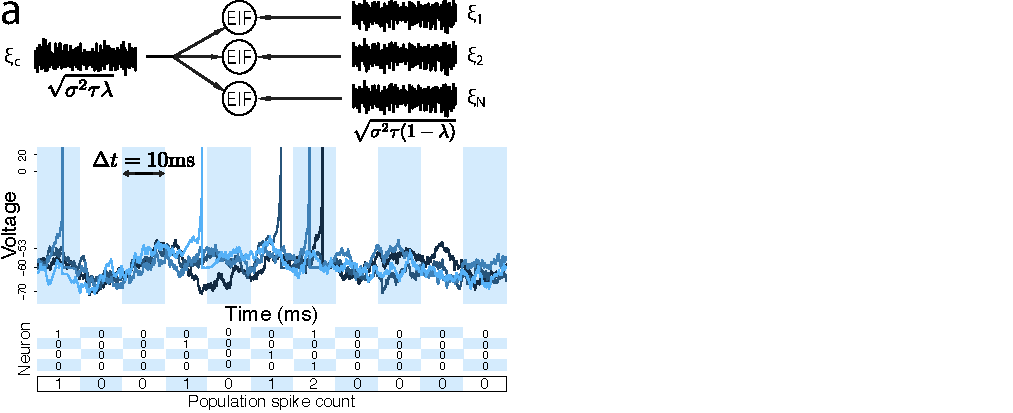
\includegraphics{figures/EIF_schematic}
\caption{\label{fig:schematic} (a) EIF neurons receiving common $\xi_c$ and independent inputs $\xi_i$. The voltages of the neurons evolve according to Eqn.~\eqref{eifsde}. Here, $\tau_m$ is the membrane time constant set as $\tau_m = 5$ms, $\Delta_T$ controls the slope of the action potential initiation, taken to be $3$mV. The EIF neuron has a ``soft'' threshold, $V_S$ of $-53$mV. Time is divided into bins of $10$ms. A spike occurs when the voltage reaches a threshold $V_T$ of $20$mV. The voltage is reset to the resting potential $V_R$ of $-60$mV and another spike cannot occur during the refractory period $\tau_{\text{ref}}$ of $3$ms. (b) A cartoon of the binning process: spikes recorded from each of the EIF neurons in a bin contribute towards the population spike count. More than one spike occurring {\em from the same neuron} within a single bin is treated as a single event. This happens less than $0.4\%$ of the time in our numerical simulations with $\mu=0.1$ and $\rho=0.1$. We tune the noise amplitude so that when the DC component of the input is set to be $\gamma = -60$mV, the neurons fire at $10$Hz; this yields $\sigma = 6.23$mV.
}
\end{figure}

The input current has a constant (DC) component $\gamma$, which sets the equilibrium (rest) potential, and a stochastic noise component with amplitude $\sigma$. The input is modeled by a correlated Gaussian with mean $\gamma$, and correlation $\lambda$. 

The spikes are binned with temporal resolution $T_\text{bin}$, which we choose to be $10$ms. On rare occasions ($<0.4\%$ of bins, see Fig.~\ref{fig:schematic} caption) multiple spikes from the same neuron can occur in the same bin. These are considered as a single spike. The output firing rate of is quantified by $\mu$, the probability of a spike occurring in a bin. Pairwise correlations between the spiking in simultaneous bins of different neurons is quantified by the correlation coefficient $\rho=\alpha/\mu(1-\mu)$, where $\alpha$ is the corresponding covariance.
%%%%
% EIF %
%%%%

\paragraph*{Emergence of strong higher-order correlations:} As in~\cite{Macke,Barreiro,Panzeri,Amarietal03}, we describe the network-wide firing statistics via the distribution of population spike counts (i.e.,~the number of simultaneously firing cells out of a maximum of $N$). The population spike count distribution is strongly skewed see Fig.~\ref{fig:eifising}(a). Do beyond-pairwise correlations plan an important role in determining this structure? To answer this, we compare the population spike-count distributions for the EIF model and its second-order approximation via a pairwise maximum entropy model, where the probability of the population spike count having $k$ active neurons out of a total $N$ is: $P_{\text{PME}}(k) = Z^{-1} \binom{N}{k}\exp{(\alpha k + \beta k^2)}$, for details see~\cite{Macke2011}. For small populations the PME does a satisfactory job. For populations larger than about $N=30$ neurons the PME fails to capture the shape of the distribution: Fig.~\ref{fig:eifising}(a). 
%%%%%%%%%%%%%%
\begin{figure}[h]
\includegraphics{figures/fig_2a.pdf}
\caption{\label{fig:eifising}(a) Population spike-count distributions for the EIF model and its second-order approximation for $8, 32, 64, \text{and } 100$ neurons for $\mu = 0.1$ and $\rho = 0.1$. The distributions are similar for smaller populations and different for large populations. Inset: the same distributions on a log-linear scale. (b) The Jensen-Shannon (JS) divergence between the EIF and the pairwise maximum entropy (PME) model. We normalize by $\log(N)$, which is the natural growth rate of the JS-divergence with population. (Left) JS-divergence for a constant value of $\mu = 0.1$ and increasing values of $\rho$, and (Right) for constant value of $\rho = 0.1$ and increasing values of $\mu$ as the population size increases. The JS-divergence grows with increasing correlation $\rho$ and decreasing mean firing rate $\mu$.}
\end{figure}
%%%%%%%%%%%%%%

We quantify the divergence between the PME and EIF population output distributions via the normalized JS-divergence, see Fig.~\ref{fig:eifising}(b). The EIF model produces strong beyond-pairwise correlations at a wide range of correlations $\rho$ and mean firing rates $\mu$. Additionally, as in~\cite{Macke, cf. Roudi}, the Jensen-Shannon divergence grows with increasing population size $N$. Moreover, the divergence increases with increasing pairwise correlation and decreasing mean firing rate.

%%%%
% LNL %
%%%%

%%%%%%%%%%%%%%%%%%
\begin{figure}[t!]
\includegraphics{figures/fig_3a}
\caption{\label{fig:linearfilter} (a) The linear filter $A(t)$ and static non-linearity for several values of the correlation coefficient $\rho$. The filter receives a noise amplitude of $\sigma\sqrt{1-\lambda}$. The static-nonlinearity receives a noise amplitude of $\sigma$. (b) The static non-linearity applied to the linear estimate of the firing rate, for $\mu = 0.1$, $\rho = 0.1$. The non-linearity increases the firing rate magnitude and rectifies negative firing rates.}
\end{figure}
%%%%%%%%%%%%%%%%%

\paragraph*{A semi-analytic spiking model that produces higher-order correlations.} We next derive a semi-analytical approximation for the EIF population statistics based on linear response theory. This is a linear-nonlinear cascade, where each neuron fires as an inhomogeneous Poisson process with rate given by convolving a temporal filter $A(t)$ with an input signal $c(t)$ and then applying a time independent nonlinear function \cite{Ostoijic} $F$:   
\begin{equation}
r(t) = F\left(A * c(t) \right). \nonumber
\end{equation}
The signal for each cell is the common input, so that $c(t) = \sqrt{\sigma^2 \tau \lambda}~\xi_c(t)$. The filter $A(t)$ is computed as the linear response of the firing rate to a weak input signal, via an expansion of the Fokker Planck equation for Eqn.~\eqref{eifsde} around the equilibrium obtained with ``background'' current $\gamma+ \sqrt{\sigma^2 \tau (1-\lambda)}~\xi(t)$ . This calculation follows exactly the methods described in \cite{Richardson}. For the static nonlinearity, we follow \cite{Ostojic:2011} and take $F(x) = \Phi\left( \gamma + \frac{x}{\Phi^\prime(\gamma)}\right)$, where $\Phi\left( \gamma \right)$ is the equilibrium firing rate obtained at the background currents described above.  This choice, in particular, ensures that we recover the linear approximation $r(t) = A * c(t)$ for weak input signals. The linear filter must be approximated numerically hence the semi-analytic nature of our model. The numerical approximations for the filter, nonlinearity, and resulting firing rate are shown in Fig.~\ref{fig:linearfilter}.

%%%%%%%%%%%%%%
\begin{figure}[h]
\includegraphics{figures/fig_4a}
\caption{\label{fig:eiffilter} The linear-nonlinear cascade gives a good approximation of the EIF population distributions. (a) A comparison between the population spike-count distributions for the EIF model and the linear-nonlinear cascade approximation for $8,~32,~64,~\text{and } 100$ neurons for $\mu = 0.1$ and $\rho = 0.1$. The LNL model greatly overestimates the zero population spike count probabilities. One reason is that there is no refractory period. The LNL model underestimates the tails of the probability distributions. This is because of the double counting, when truncating spikes in a bin the larger spike counts are penalized to a greater extent. Inset: the same distributions on a log-linear scale. (b) JS-divergence, order of magnitude smaller than PME, possibly converges to some limit? The order of the mean firing rates is reversed when compared to the PME because the LNL cascade gives a better approximation at higher firing rates $\mu$, less problems with negative firing rates...}
\end{figure}
%%%%%%%%%%%%%%%


For an inhomogeneous Poisson process with rate $r(t)$ conditioned on a common input $c(t)$ the probability of at least one spike occurring in the interval $[t,t+\Delta t]$ is:
\begin{equation*}
P(\text{spike}\in\Delta t | c ) = 1 - \exp{\left(-\int_0^{\Delta t} \! r(s+t) \dd s \right)} \;.
\end{equation*}
Introducing the notation  $\mathcal{S} = \int_0^{\Delta t} \! r(s) \dd s $ we see that $P(\text{spike}\in\Delta t | c ) = 1 - \exp (-\mathcal{S}) \equiv L(\mathcal{S})$.  

Conditioned on the common input -- or, equivalently, the windowed firing rate $\mathcal{S}$ -- each of the $N$ neurons produces spikes independently. Thus, the probability of $k$ cells firing simultaneously is:
\begin{equation}
P_{\text{LF}}(k) = \binom{n}{k} \int_{-\infty}^{~\infty} \phi_{LF}(\mathcal{S}) \big(1-\tilde{L}\big)^{n-k} \tilde{L}^{k} \dd \mathcal{S},
\end{equation}
where $\phi_{LF}(\mathcal{S})$ is the probability density function for $\mathcal{S}$.  We estimate $\phi_{LF}$ numerically.


\begin{figure*}
\includegraphics{figures/fig_5}
\caption{\label{fig:lnldgcomp} (a) The Dichotomized Gaussian (DG) model gives an excellent description of the exponential integrate-and-fire (EIF) population spike count probability distributions across a range of correlation coefficient values. The two models are plotted on top of one another and appear as a single curve for each value of $\rho$. (b) Comparing the $L(s)$ function for the DG and the $\tilde{L}(s)$ function for the EIF (after transforming from the EIF probability density function for the variable $\mathcal{S}$ to the DG variable $s$. The functions agree to an extent over the pdf $\phi_DG$ of the DG model. The DG function $L(s)$ tends to $0$ for negative values of $s$ where the LNL function $\tilde{L}(s)$ tends to a finite non-zero value. This agrees with the probability distributions in the previous model where the LNL cascade is less accurate at estimating the $0$-population spike count and large population spike count probabilities. (c) The heat capacity increases linearly for the LNL-cascade, the EIF and the DG. For the case of the LNL cascade the heat capacity increases at a slightly greater rate than the EIF/DG which overlap. The Ising model saturates for a population of approximately $N=30$ neurons.}
\end{figure*}
%For the linear estimate, when the static-nonlinearity is the identity $F(L) = L$, the variable $\mathcal{S}$ is Gaussian with $\mathbb{E}(\mathcal{S}) = 0$, $\mathbb{E}(\mathcal{S}^2) = \sigma^2 \tau_m \lambda \int_{-\infty}^{\infty} B^2 (\tau) \dd \tau$, where $B(\tau) = \int_0^{\Delta t} A(t-\tau) \dd t$. However when using the non-linearity, the variable $\mathcal{S}$ is no longer Gaussian and its statistics must be evaluated numerically.
%In terms of this variable $\mathcal{S}$ the neurons are conditionally independent and the probability of observing a spike count $k$ is:
%\begin{equation}
%P_{\text{LF}}(k) = \binom{n}{k} \int_{-\infty}^{~\infty} \phi_{LF}(\mathcal{S}) \big(1-\tilde{L}\big)^{n-k} \tilde{L}^{k} \dd \mathcal{S}
%\end{equation}
%where $\tilde{L}(\mathcal{S}) = 1-\exp(-\mathcal{S})$, and $\phi_{LF}(\mathcal{S})$ is the probability density function of the integral of the firing rate over a time bin.

%Unlike the full EIF model, by using this analytical calculation there are no problems with doubly binned spikes.

%%%%
% DG %
%%%%

%%%%%%%%%%%
% LNL CASCADE    %
%%%%%%%%%%%

Figure~\ref{fig:eiffilter}(a) shows that the LNL cascade captures the general structure of the EIF population output across a range of population sizes.  In particular, it produces an order-of-magnitude improvement over the PME model (see DJS values in Fig.~\ref{fig:eiffilter}(b)), and reproduces the skewed structure produced by beyond-pairwise correlations.  

This said, the LNL model does not produce a perfect fit to the EIF outputs, the most obvious problem being the overestimation of the zero spike probabilities, which $N=100$ case are overestimated by almost $100\%$ (the tail probabilities are also underestimated).
Notably, the LNL fits become almost perfect for lower correlations i.e.~$\rho = 0.05$ (see supplemental material \Ecomment{Can we add such a panel for N=100 to supplemental ... like the N=100 histograms, but for rho=0.05?}). This suggests the errors are due to the way the static non-linearity deals with fluctuations to very low or high firing rates $r(t)$; these fluctuations are smaller at lower correlation values, which lead to smaller signal currents in the LNL formulation.  

%nstantaneous. This leads to large periods of very low firing rates of less than $1$Hz. We find that for $\rho = 0.05$ the linear estimate of the firing rate is negative $20\%$ of the time , and $30\%$ of the time for $\rho=0.1$. By examining the $\tilde{L}(\mathcal{S})$ function we also get some clues.
%
%The LNL cascade also underestimates the tails of the probability distributions. Maybe the higher frequency estimate of the firing rate is too low? Maybe it's not at a high enough firing rate for long enough? There is a way to fix this in the numerical simulations but not in the theory. In the numerical simulations you can allow extra spikes in a bin to contribute to the total. Maybe it's because the nonlinearity saturates at a value that is too low.
%
%The JS-divergence between the EIF model and the LNL model is an order of magnitude better than the PME model figure 3(b). The order of the mean firing rate order is reversed when compared to the EIF model. Does it look like it's converging? Can we do $N=200$? 




\paragraph*{Relating the EIF and Dichotomous Gaussian models}

The LNL model provides a reduction of the EIF model to an inhomogeneous poisson process that is based directly on the underlying SDEs.  In many settings -- and especially in experiments -- we seek more abstracted statistical models of spike outputs.  We now demonstrate that one such approach, which has been shown to produce ~\cite{Amari,Macke} and capture ~\cite{Yu} higher-order correlations before, reproduces the EIF population activity with exquisite accuracy.  

In this Dichotomous Gaussian framework, introduced by~\cite{Amari,Macke}, $N$ neurons receive correlated Gaussian input with mean $\gamma$ and covariance $\lambda$. Each neuron applies a step nonlinearity to its inputs, spiking only if its input is positive. The mean of the input is chosen so that the mean of the output is $\mu$ and similarly $\lambda$ is chosen so that the correlation coefficient is $\rho$.
The correlated Gaussian can be written as: $Z_i = \gamma + \sqrt{1-\lambda} T_i + \sqrt{\lambda} S$ where $T_i$ is the independent input and $S$ is the common input. The probability of a spike is given by $P(Z_i > 0 | s)$ and again we can define the $L(s)$ function:  \Ecomment{check lower case vs upper case s usage}
\begin{equation}
L(s) = P\left( T_i > \frac{-s-\gamma}{\sqrt{1-\lambda}} \right) = \Phi\left(\frac{s+\gamma}{\sqrt{1-\lambda}}\right)
\label{e.Ldg}
\end{equation}
\Ecomment{$\Phi$ used differently in diff parts of paper -- use different choice for LNL model?}
Equipped with Eqn.~\eqref{e.Ldg}, the probability of observing a spike count $k$ is the same as equation [eqnum] using $L(s)$ and $\phi_{DG}(s)$ is the probability density function of a one-dimensional Gaussian with mean $0$ and variance $\lambda$.

Fig.~\ref{fig:lnldgcomp}a shows that the Dichotomized Gaussian model provides an essentially exact description of the EIF population output for a range of firing statistics.
% probability distributions of the EIF neurons receiving common input, see  where the EIF model distribution is plotted alongside the DG prediction for $N=100$ neurons for various correlation coefficients at a mean firing rate of $\mu = 0.1$. To see why this is the case we use the LNL cascade model to see how the models are similar.
We evaluate this connection to the EIF model via the probability distributions $P_{\text{LNL}}$ and $P_{\text{DG}}$. To make the comparison we must transform from the probability density function of the linear-nonlinear model $\phi_{LF}$ to the Gaussian pdf $\phi_{DG}$ using the nonlinear change of variable:
\begin{equation}
\mathcal{S} = f(s),\quad\text{where}\quad f^\prime(s) = \frac{\phi_{DG}(s)}{\phi_{LF}\big(f(s)\big)}.
\end{equation}
Writing the LNL cascade probability in terms of the $s$ variable we get:
\begin{equation}
P_{\text{LF}}(k) = \binom{n}{k}\!\!\int_{-\infty}^{~\infty} \phi_{\text{DG}}(s) \big(1-\tilde{L}(f(s))\big)^{n-k} \tilde{L}(f(s))^{k} \dd s
\end{equation}
where $\tilde{L}(\mathcal{S}) = 1-\exp(-\mathcal{S})$. After this transformation the only difference between the models is now the $L(s)$ functions. The comparison between $L$ and $\tilde{L}$ can be seen in figure 4(b). The functions largely agree over about $2$ standard deviations of the Gaussian pdf of values of the common input signal $s$.  At large values of common input $s$, the higher values of the DG $L(s)$ account for the more accurate fit of the tail of $P(k)$ \Ecomment{Need to make sure phrasing and references to symbols here make sense.}  

The success of the DG model in capturing EIF statistics is significant for two reasons.  First, it suggests why this abstracted model has been able to capture the population output recorded from spiking neurons.  Second, because the DG model is a special case of a Bernoulli generalized linear model (see supplemental material), our finding indicates that this very broad and easily fittable class of statistical models may be able to capture the higher-order population activity in neural data.   

\bigskip



\bigskip

\Ecomment{Add discussion of heat capacity ... }

\bigskip 
{\it Summary and conclusion:}   %
%%%%%%%%%%%%
We have shown that Exponential-Integrate and Fire (EIF) neurons receiving common input give rise to strong higher-order correlations.  Moreover, the correlation structure that results can be predicted from a linear-nonlinear cascade model, which forms  a tractable reduction of the EIF neuron.  Overall, the cascade model gives an order of magnitude better description of the EIF population spike count distribution and provides a simple mechanism for higher-order correlations.  Moreover, this model can be directly related to the Dichotomized Gaussian model , which has been highly successful in the experimental and statistical literature.

\bigskip 

\bigskip



The authors thank Liam Paninski for helpful insights. This work was supported by the Burroughs Wellcome Fund Scientific Interfaces Program and NSF Grants DMS-xxxx and CAREER-xxxxx.  

\bibliographystyle{plain}
\bibliography{HOC_bib}% Produces the bibliography via BibTeX.

\newpage
.
\newpage

\Ecomment{Eventually break this off and submit as separate file ... typeset with single column }


\bigskip

SUPPLEMENTARY MATERIAL 

\bigskip


{\it Relating DG and Generalized Linear models:}
The LNL model provides a reduction of the EIF model to an inhomogeneous poisson process that is based directly on the underlying SDEs, and is in extremely wide use in neural modeling~\cite{Abb-Dayan}.  However, it far from the only approach to statistical modeling of spiking neurons.  In particular, generalized linear models can be fit to the Bernoulli data given by the 1's and 0's of binned spikes in individual cells.  Such models similarly apply a linear filter to the common input signal, and followed by a static nonlinearity $f(\cdot)$, to yield a spiking probability for the current time bin.  Noting that any linear filter on our (gaussian white noise) input signal will yield a gaussian value $s$, this class of models therefore yields spiking probabilities $f(s)$ where $s$ is gaussian.  Comparing with Eqn.~\eqref{e.Ldg} in the main text, we see that the DG and GLM models have the same general form, when $f$ is taken to be the cumulative distribution function for a gaussian (as in ``probit" models). 


\end{document}
%
% ****** End of file apssamp.tex ******
